\documentclass[11pt,a4paper]{article}

\usepackage[utf8]{inputenc}
\usepackage[T1]{fontenc}
\usepackage[french]{babel}
\usepackage{amsmath,amssymb}
\usepackage{graphicx}
\usepackage[a4paper,margin=2.5cm]{geometry}
\usepackage{hyperref}
\hypersetup{colorlinks=true,linkcolor=black,urlcolor=blue,citecolor=black}

% Mise en page un peu plus aeree : interligne et espacement entre paragraphes.
\linespread{1.05}
\setlength{\parskip}{0.6em}

\graphicspath{{figures/}}

\title{Projet Méthodes Stochastiques\\[0.3em]
       \large Modèle proie-prédateur avec virus}
\author{Philippe \textsc{Lin} \and Sayna \textsc{Ren} \and Xuhong \textsc{Liu}}
\date{}

\begin{document}

\maketitle

\textit{Tous les résultats présentés dans ce rapport sont reproductibles dans le notebook qui l'accompagne, où l'on trouve également l'ensemble des codes.}

\section*{Contexte et modèle}

On étudie la dynamique de deux populations en interaction, les victimes (les proies) de densité $V_t$ et les prédateurs de densité $P_t$. Le point de départ est le modèle de Lotka-Volterra où les proies se reproduisent seules mais se font manger par les prédateurs tandis que les prédateurs meurent naturellement mais profitent de l'abondance des proies pour se reproduire.

Lorsqu'aucune perturbation extérieure n'intervient, cette dynamique s'écrit comme un système de Lotka-Volterra déterministe, avec $a$, $b$, $c$ et $d$ des coefficients positifs.

\begin{equation}\label{eq:base}
  dV_t = V_t\left(a - b\,P_t\right)dt,
  \qquad
  dP_t = P_t\left(-c + d\,V_t\right)dt.
\end{equation}

Un tel système admet des solutions périodiques si bien que les deux populations oscillent indéfiniment autour de leur point d'équilibre.

\section*{Question 1 — Proposer et valider un modèle pour le virus}

Dans le jeu de données \texttt{virus4.csv}, les proies sont en plus frappées par un virus que l'on modélise par un processus stochastique $(X_t)_{t\in[0,\tau]}$. Le système devient alors

\begin{equation}\label{eq:systeme}
  dV_t = V_t\left(\tfrac{2}{3} - \tfrac{4}{3}P_t + X_t\right)dt,
  \qquad
  dP_t = P_t\left(-1 + V_t\right)dt.
\end{equation}

Le fichier fournit une observation discrétisée de cette dynamique dont la première colonne correspond à $V_t$ et la seconde à $P_t$. Notre objectif est de proposer un modèle pour $(X_t)$ puis de le valider à l'aide de ces données.

Avant de nous lancer dans la modélisation, il nous a semblé naturel de commencer par regarder les données pour voir à quoi ressemblent les deux populations au cours du temps et en quoi elles s'écartent du modèle déterministe. Nous espérions ainsi nous faire une première idée de ce que le virus fait réellement au système.

\subsection*{Récupération du pas de temps}

Le fichier contient $2000$ points mais nous ne connaissions pas a priori le pas de temps de la discrétisation. Une idée a été d'exploiter le fait que l'équation des prédateurs ne contient aucun bruit puisque l'on a exactement $dP_t = P_t(-1 + V_t)\,dt$. En discrétisant, le pas de temps devrait alors vérifier

\begin{equation}\label{eq:dt}
  dt \approx \frac{P_{i+1} - P_i}{P_i\,(-1 + V_i)}.
\end{equation}

Nous avons donc moyenné cette quantité sur l'ensemble des points tout en écartant ceux où $V_i$ est trop proche de $1$ parce qu'ils annulent le dénominateur. On obtient ainsi $dt \approx 0{,}015$, ce qui donne une durée d'observation $\tau = 2000 \times 0{,}015 = 30$. Cela nous a permis de construire l'axe des temps puis de tracer les deux populations (figure~\ref{fig:series}).

\begin{figure}[ht]
  \centering
  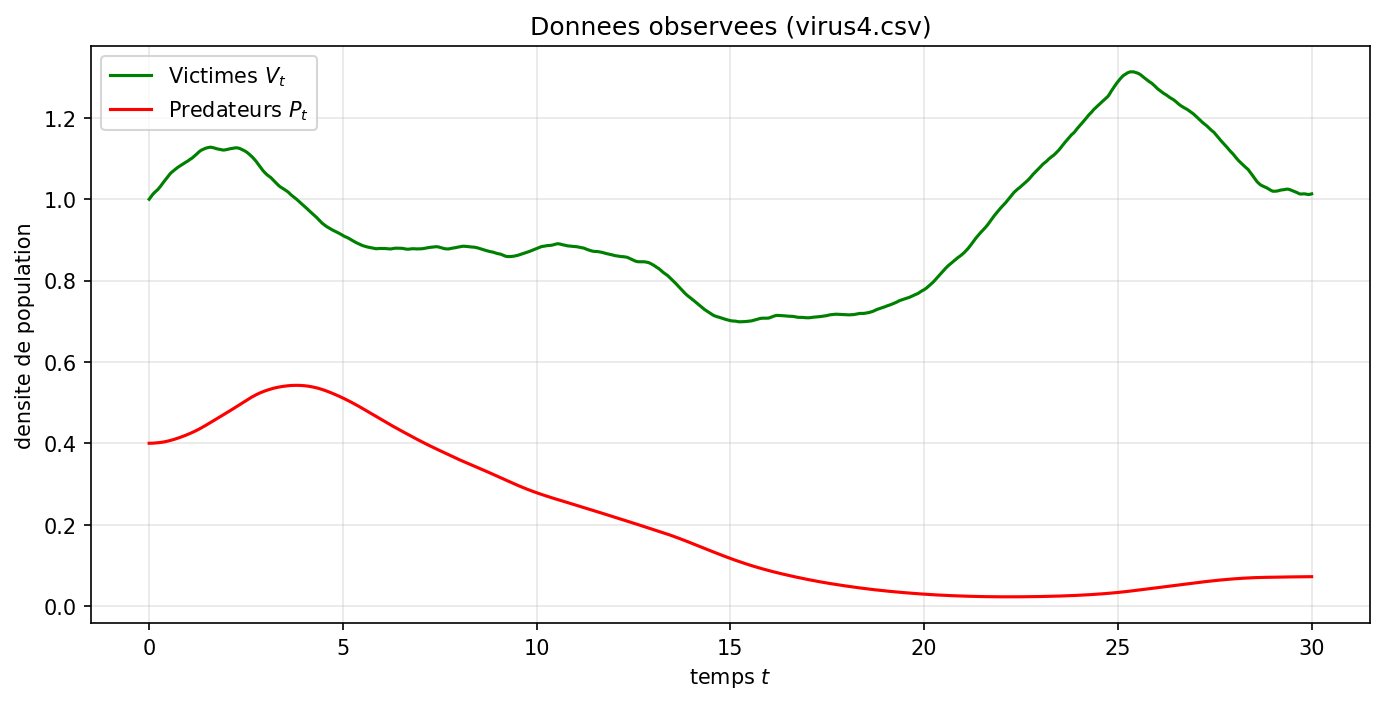
\includegraphics[width=0.85\textwidth]{virus4_series.png}
  \caption{Évolution observée des densités de victimes $V_t$ et de prédateurs $P_t$ sur l'intervalle $[0,\tau]$, reconstruite à partir de \texttt{virus4.csv}.}
  \label{fig:series}
\end{figure}

\subsection*{Comparaison avec le modèle de Lotka-Volterra classique}

Pour essayer de mesurer l'effet du virus, nous avons eu l'idée d'intégrer le modèle déterministe classique, c'est-à-dire le même système lorsque l'on retire le terme $X_t$. Une petite identification avec la forme générale~\eqref{eq:base} donne $a = \tfrac{2}{3}$, $b = \tfrac{4}{3}$, $c = 1$ et $d = 1$. Nous sommes partis des mêmes conditions initiales que les données, soit $V_0 = 1$ et $P_0 = 0{,}4$. La figure~\ref{fig:comparaison} superpose les deux trajectoires.

\begin{figure}[ht]
  \centering
  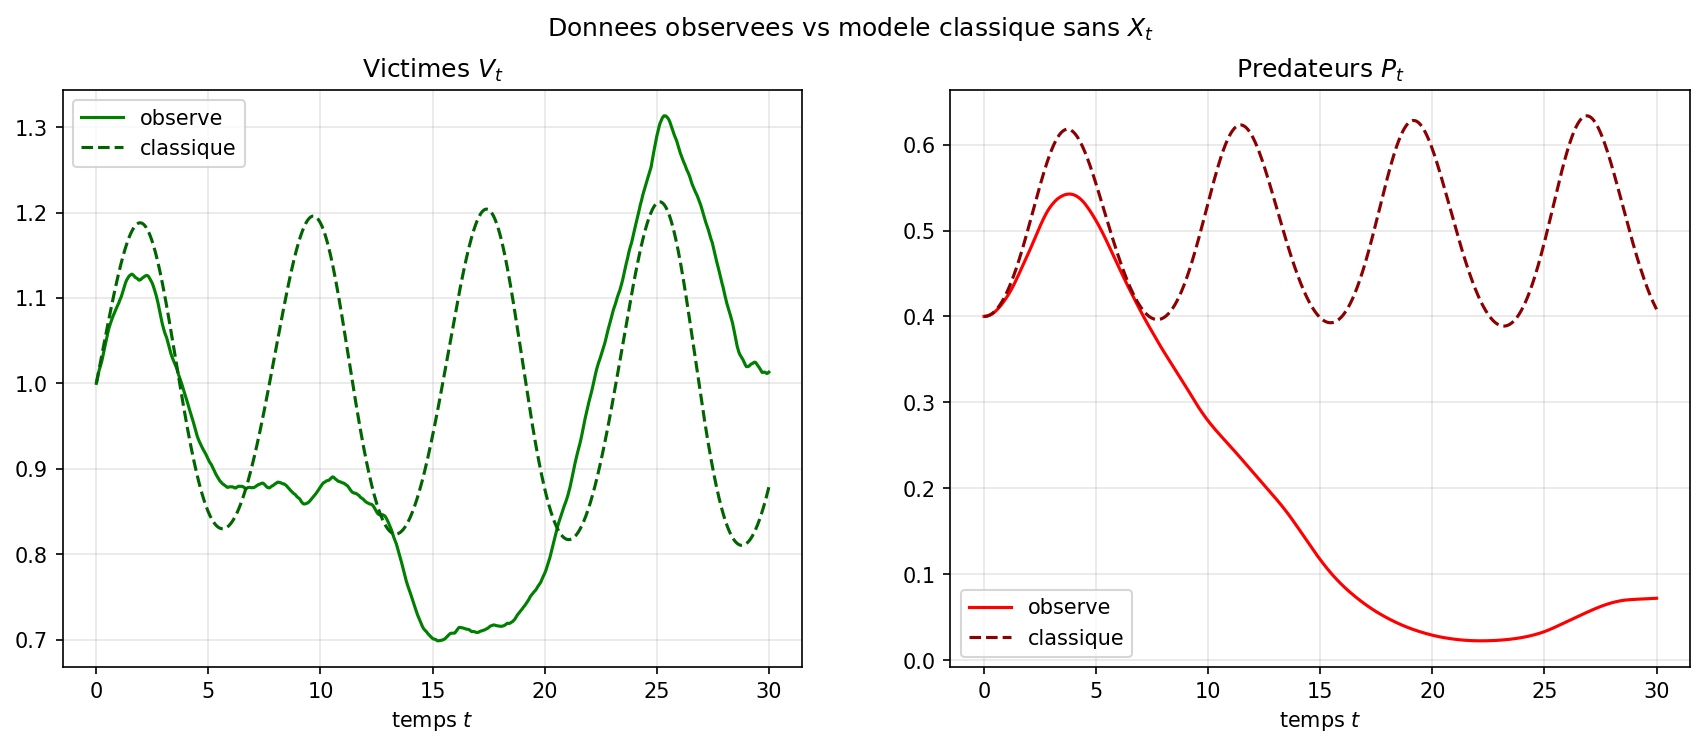
\includegraphics[width=\textwidth]{virus4_comparaison.png}
  \caption{Comparaison entre les données observées (trait plein) et le modèle de Lotka-Volterra classique sans $X_t$ (tirets), pour les victimes (gauche) et les prédateurs (droite).}
  \label{fig:comparaison}
\end{figure}

\subsection*{Premières observations}

La comparaison nous a semblé parlante. Le modèle classique produit des oscillations régulières et entretenues où les deux populations tournent indéfiniment autour de leur point d'équilibre et où le portrait de phase serait une courbe fermée bien nette. Les données observées partent dans la même direction au tout début mais s'en écartent franchement ensuite. La population de prédateurs ne semble notamment pas ré-osciller puisqu'elle s'effondre progressivement et reste très basse alors que le modèle classique la voit remonter à chaque cycle.

Nous en avons retiré l'impression que le terme de virus $X_t$ ne se contente pas d'ajouter un petit bruit autour de la trajectoire classique mais qu'il modifie la dynamique d'ensemble et casse la périodicité. C'est sur ce comportement que nous avons choisi d'appuyer la modélisation de $(X_t)$ dans la suite.

\subsection*{Reconstruction du virus $X_t$}

Intéressons-nous maintenant directement à $X_t$. En supposant que le virus admet une moyenne finie $\mu = \mathbb{E}[X_t]$ (hypothèse que nous vérifierons plus loin mais qui paraît tout à fait plausible), on peut passer l'équation des proies à sa moyenne et en chercher l'équilibre. Le taux de croissance moyen des proies s'annule lorsque $\tfrac{2}{3} - \tfrac{4}{3}P_t + \mu = 0$, ce qui déplace l'équilibre des prédateurs du cas classique $P^* = \tfrac{1}{2}$ vers

\begin{equation}\label{eq:equilibre}
  P^* = \frac{1}{2} + \frac{3}{4}\mu.
\end{equation}

Or la figure~\ref{fig:series} montre des prédateurs qui s'effondrent bien en dessous de $\tfrac{1}{2}$, donc on s'attend à une moyenne $\mu$ négative.

Pour vérifier cette intuition nous avons eu l'idée de discrétiser l'équation de $dV_t$. En remplaçant $dV_t$ par l'incrément $V_i - V_{i-1}$ et en évaluant le membre de droite au début du pas, on obtient

\begin{equation}\label{eq:disc}
  V_i - V_{i-1} \approx V_{i-1}\left(\tfrac{2}{3} - \tfrac{4}{3}P_{i-1} + X_{i-1}\right)dt.
\end{equation}

Tous les autres termes étant connus, il ne reste qu'à isoler le virus.

\begin{equation}\label{eq:xrec}
  X_{i-1} \approx \frac{V_i - V_{i-1}}{V_{i-1}\,dt} - \tfrac{2}{3} + \tfrac{4}{3}P_{i-1}.
\end{equation}

Cette reconstruction est entièrement déterministe puisqu'elle ne fait qu'inverser le schéma, sans aucune hypothèse de modèle. La figure~\ref{fig:xt} montre le virus reconstruit et ses incréments.

\begin{figure}[ht]
  \centering
  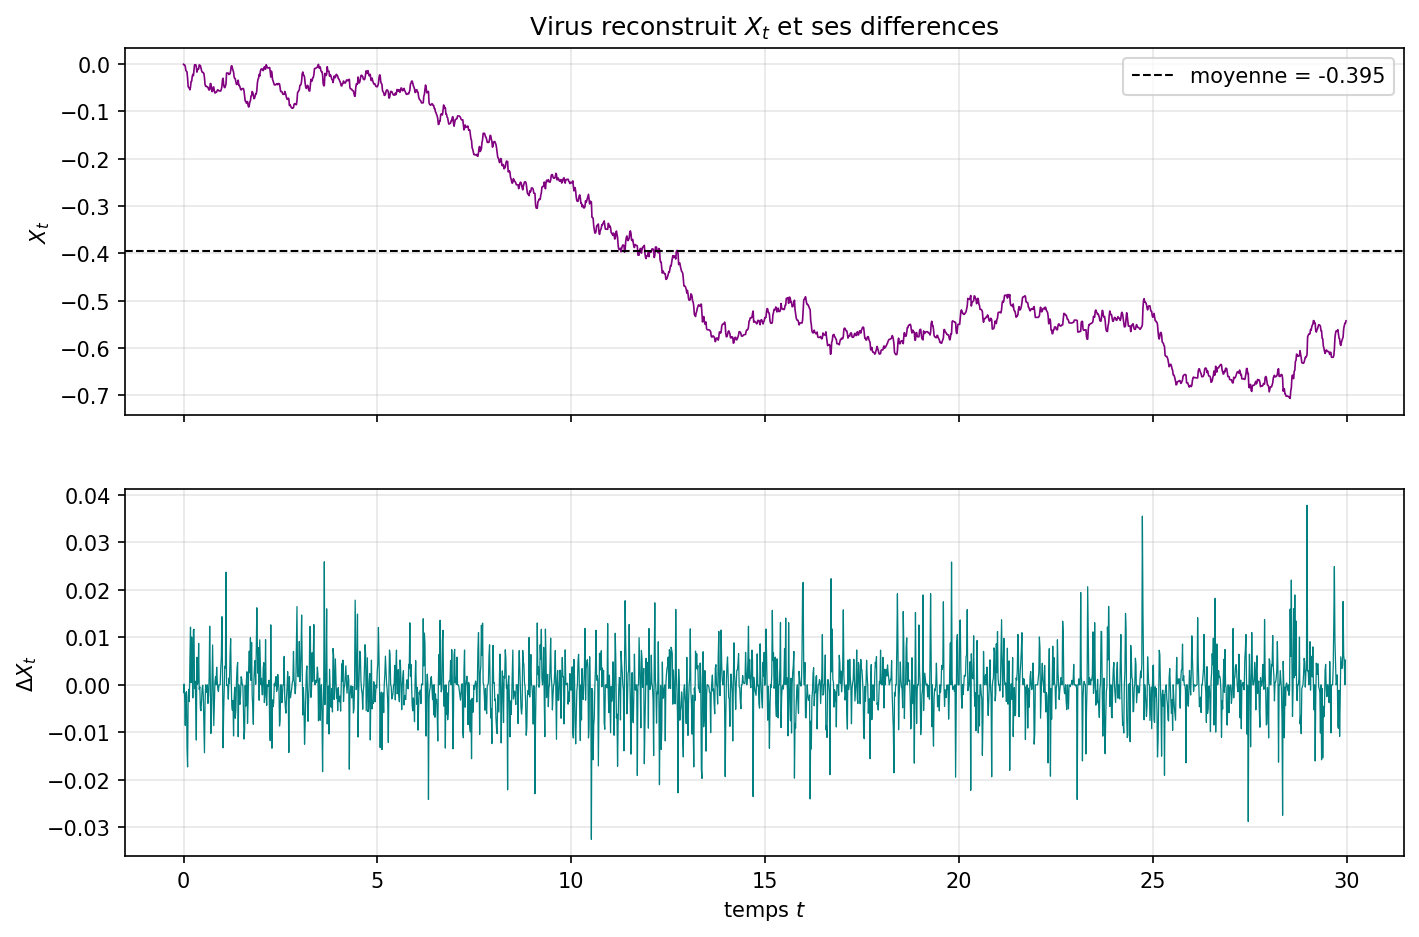
\includegraphics[width=0.9\textwidth]{virus4_Xt.png}
  \caption{En haut, le virus reconstruit $X_t$ (la moyenne empirique est en tirets). En bas, ses incréments $\Delta X_t = X_{t+dt} - X_t$.}
  \label{fig:xt}
\end{figure}

Sa moyenne empirique vaut environ $-0{,}40$, donc bien négative, ce qui confirme notre hypothèse et referme le raisonnement sur l'équilibre. Le virus part de $X_0 \approx 0$ puis décroît régulièrement jusque vers $-0{,}6$ aux alentours de $t \approx 13$ avant de se stabiliser en fluctuant. Le scénario est même plus riche qu'un simple décalage constant puisque l'intensité du virus se renforce au cours du temps, étouffant progressivement les prédateurs.

Les incréments $\Delta X_t$ ressemblent à un bruit centré d'amplitude à peu près constante, sans tendance visible. Le virus lui-même paraît donc non stationnaire sur la fenêtre observée alors que ses variations le sont. Pour préciser sa structure nous avons regardé son autocorrélation (figure~\ref{fig:xtacf}).

\begin{figure}[ht]
  \centering
  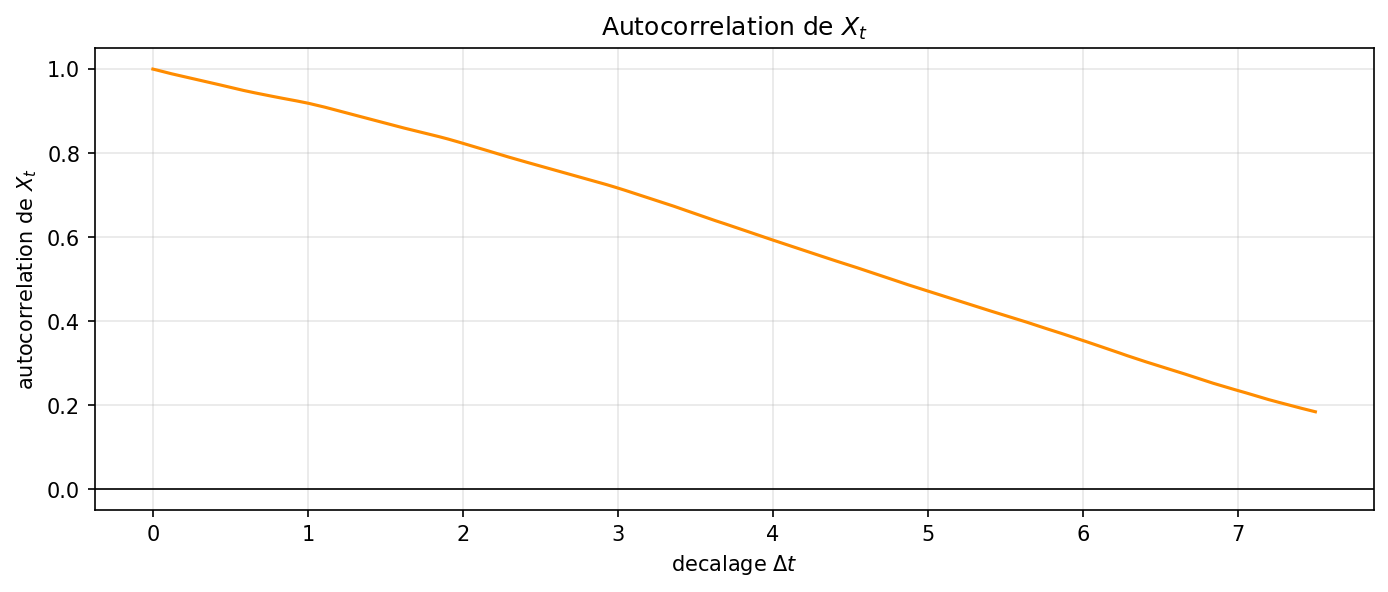
\includegraphics[width=0.85\textwidth]{virus4_Xt_acf.png}
  \caption{Autocorrélation empirique de $X_t$ en fonction du décalage.}
  \label{fig:xtacf}
\end{figure}

L'autocorrélation décroît lentement et reste forte même à grand décalage, ce qui trahit une mémoire longue plutôt qu'un retour rapide à la moyenne. Cela oriente vers une structure de type marche aléatoire (un mouvement brownien, éventuellement avec dérive) ou vers un processus à retour à la moyenne très lent. Nous n'avons pas encore tranché entre ces deux pistes, et c'est ce que nous chercherons à départager ensuite.

\end{document}